\documentclass[tikz]{standalone}
\usepackage{tikz,amsmath}
\usetikzlibrary{shapes}
\begin{document}
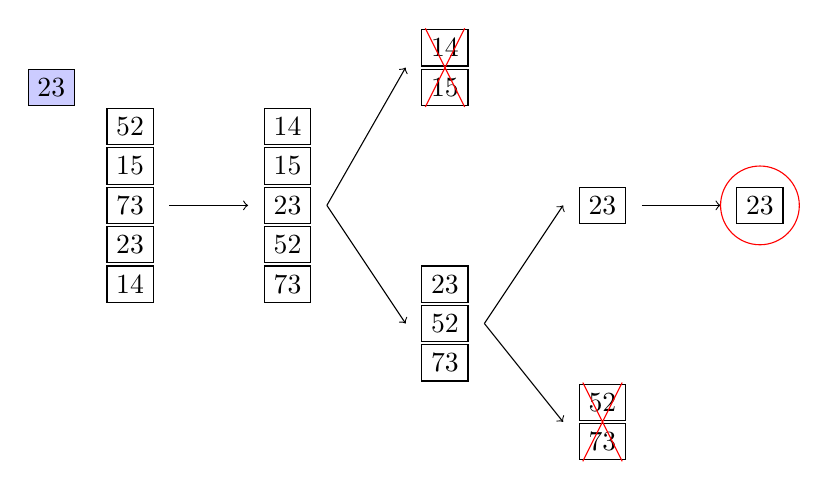
\begin{tikzpicture}
    \node [rectangle, draw, fill=blue!20] at (-1,2.5) {23};

    \node [rectangle, draw] at (0,0) {14};
    \node [rectangle, draw] at (0,.5) {23};
    \node [rectangle, draw] at (0,1) {73};
    \node [rectangle, draw] at (0,1.5) {15};
    \node [rectangle, draw] at (0,2) {52};

    \draw [->] (.5,1) -- (1.5,1);

    \node [rectangle, draw] at (2,2) {14};
    \node [rectangle, draw] at (2,1.5) {15};
    \node [rectangle, draw] at (2,1) {23};
    \node [rectangle, draw] at (2,.5) {52};
    \node [rectangle, draw] at (2,0) {73};

    \draw [->] (2.5,1) -- (3.5,2.75);
    \draw [->] (2.5,1) -- (3.5,-.5);

    \node [rectangle, draw] at (4,3) {14};
    \node [rectangle, draw] at (4,2.5) {15};
    \draw [color=red] (3.75,3.25) -- (4.25,2.25);
    \draw [color=red] (3.75,2.25) -- (4.25,3.25);

    \node [rectangle, draw] at (4,0) {23};
    \node [rectangle, draw] at (4,-.5) {52};
    \node [rectangle, draw] at (4,-1) {73};

    \draw [->] (4.5,-.5) -- (5.5,1);
    \draw [->] (4.5,-.5) -- (5.5,-1.75);

    \node [rectangle, draw] at (6,1) {23};

    \node [rectangle, draw] at (6,-1.5) {52};
    \node [rectangle, draw] at (6,-2) {73};
    \draw [color=red] (5.75,-1.25) -- (6.25,-2.25);
    \draw [color=red] (5.75,-2.25) -- (6.25,-1.25);

    \draw [->] (6.5,1) -- (7.5,1);

    \node [rectangle, draw] at (8,1) {23};
    \draw [color=red] (8,1) circle (.5);
\end{tikzpicture}
\end{document}
